\documentclass[tikz,border=10pt]{standalone}
\begin{document}
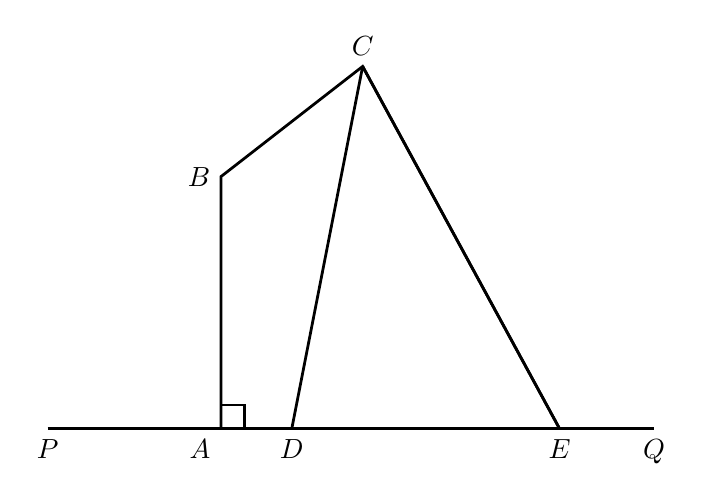
\begin{tikzpicture}[line width=1pt]
\coordinate (P) at (-2.2,0);
\coordinate (A) at (0,0);
\coordinate (D) at (0.9,0);
\coordinate (E) at (4.3,0);
\coordinate (Q) at (5.5,0);
\coordinate (B) at (0,3.2);
\coordinate (C) at (1.8,4.6);

\draw (P) -- (Q);
\draw (A) -- (B) -- (C) -- (E);
\draw (D) -- (C);
\draw (C) -- (E);
\draw (A) -- (0,0.3) -- (0.3,0.3) -- (0.3,0);

\node[below] at (P) {$P$};
\node[below left] at (A) {$A$};
\node[below] at (D) {$D$};
\node[below] at (E) {$E$};
\node[below] at (Q) {$Q$};
\node[left] at (B) {$B$};
\node[above] at (C) {$C$};
\end{tikzpicture}
\end{document}
